%	PACKAGES AND OTHER DOCUMENT CONFIGURATIONS

\documentclass[11pt, a4paper]{article} % 10pt font size (11 and 12 also possible), A4 paper (letterpaper for US letter) and two column layout (remove for one column) Use additional titlepage argument to generate this
%\documentclass[12pt, a4paper,twocolumn,titlepage]{article}

%%%%%%%%%%%%%%%%%%%%%%%%%%%%%%%%%%%%%%%%%
% Wenneker Article
% Structure Specification File
% Version 1.0 (28/2/17)
%
% This file originates from:
% http://www.LaTeXTemplates.com
%
% Authors:
% Frits Wenneker
% Vel (vel@LaTeXTemplates.com)
%
% License:
% CC BY-NC-SA 3.0 (http://creativecommons.org/licenses/by-nc-sa/3.0/)
%
%%%%%%%%%%%%%%%%%%%%%%%%%%%%%%%%%%%%%%%%%

%----------------------------------------------------------------------------------------
%	PACKAGES AND OTHER DOCUMENT CONFIGURATIONS
%----------------------------------------------------------------------------------------

\usepackage[english]{babel} % English language hyphenation

\usepackage{microtype} % Better typography

\usepackage{verbatim} % Allows mulitline commenting

\usepackage{amsmath,amsfonts,amsthm} % Math packages for equations

\usepackage[svgnames]{xcolor} % Enabling colors by their 'svgnames'

\usepackage[hang, small, labelfont=bf, up, textfont=it]{caption} % Custom captions under/above tables and figures

\usepackage{subcaption}

\usepackage{booktabs} % Horizontal rules in tables

\usepackage{lastpage} % Used to determine the number of pages in the document (for "Page X of Total")

\usepackage{graphicx} % Required for adding images

\usepackage{enumitem} % Required for customising lists
\setlist{noitemsep} % Remove spacing between bullet/numbered list elements

\usepackage{sectsty} % Enables custom section titles
\allsectionsfont{\usefont{OT1}{phv}{b}{n}} % Change the font of all section commands (Helvetica)

\usepackage{siunitx}

%----------------------------------------------------------------------------------------
%	MARGINS AND SPACING
%----------------------------------------------------------------------------------------

\usepackage{geometry} % Required for adjusting page dimensions

\geometry{
	top=1cm, % Top margin
	bottom=1.5cm, % Bottom margin
	left=2cm, % Left margin
	right=2cm, % Right margin
	includehead, % Include space for a header
	includefoot, % Include space for a footer
	%showframe, % Uncomment to show how the type block is set on the page
}

\setlength{\columnsep}{7mm} % Column separation width

%----------------------------------------------------------------------------------------
%	FONTS
%----------------------------------------------------------------------------------------

\usepackage[T1]{fontenc} % Output font encoding for international characters
\usepackage[utf8]{inputenc} % Required for inputting international characters

\usepackage{XCharter} % Use the XCharter font

%----------------------------------------------------------------------------------------
%	HEADERS AND FOOTERS
%----------------------------------------------------------------------------------------

\usepackage{fancyhdr} % Needed to define custom headers/footers
\pagestyle{fancy} % Enables the custom headers/footers

\renewcommand{\headrulewidth}{0.0pt} % No header rule
\renewcommand{\footrulewidth}{0.4pt} % Thin footer rule

\renewcommand{\sectionmark}[1]{\markboth{#1}{}} % Removes the section number from the header when \leftmark is used

%\nouppercase\leftmark % Add this to one of the lines below if you want a section title in the header/footer

% Headers
\lhead{} % Left header
\chead{\textit{\thetitle}} % Center header - currently printing the article title
\rhead{} % Right header

% Footers
\lfoot{} % Left footer
\cfoot{} % Center footer
\rfoot{\footnotesize Page \thepage\ of \pageref{LastPage}} % Right footer, "Page 1 of 2"

\fancypagestyle{firstpage}{ % Page style for the first page with the title
	\fancyhf{}
	\renewcommand{\footrulewidth}{0pt} % Suppress footer rule
}

%----------------------------------------------------------------------------------------
%	TITLE SECTION
%----------------------------------------------------------------------------------------

\newcommand{\authorstyle}[1]{{\large\usefont{OT1}{phv}{b}{n}\color{NavyBlue}#1}} % Authors style (Helvetica)

\newcommand{\institution}[1]{{\footnotesize\usefont{OT1}{phv}{m}{sl}\color{Black}#1}} % Institutions style (Helvetica)

\usepackage{titling} % Allows custom title configuration

\newcommand{\HorRule}{\color{SteelBlue}\rule{\linewidth}{1pt}} % Defines the gold horizontal rule around the title

\pretitle{
	\vspace{-30pt} % Move the entire title section up
	\HorRule\vspace{10pt} % Horizontal rule before the title
	\fontsize{32}{36}\usefont{OT1}{phv}{b}{n}\selectfont % Helvetica
	\color{Navy} % Text colour for the title and author(s)
}

\posttitle{\par\vskip 15pt} % Whitespace under the title

\preauthor{} % Anything that will appear before \author is printed

\postauthor{ % Anything that will appear after \author is printed
	\vspace{10pt} % Space before the rule
	\par\HorRule % Horizontal rule after the title
	\vspace{20pt} % Space after the title section
}

%----------------------------------------------------------------------------------------
%	ABSTRACT
%----------------------------------------------------------------------------------------

\usepackage{lettrine} % Package to accentuate the first letter of the text (lettrine)
\usepackage{fix-cm}	% Fixes the height of the lettrine

\newcommand{\initial}[1]{ % Defines the command and style for the lettrine
	\lettrine[lines=3,findent=4pt,nindent=0pt]{% Lettrine takes up 3 lines, the text to the right of it is indented 4pt and further indenting of lines 2+ is stopped
		\color{NavyBlue}% Lettrine colour gold DarkGoldenRod
		{#1}% The letter
	}{}%
}

\usepackage{xstring} % Required for string manipulation

\newcommand{\lettrineabstract}[1]{
	\StrLeft{#1}{1}[\firstletter] % Capture the first letter of the abstract for the lettrine
	\initial{\firstletter}\textbf{\StrGobbleLeft{#1}{1}} % Print the abstract with the first letter as a lettrine and the rest in bold
}

%	BIBLIOGRAPHY

\usepackage[backend=biber,style=phys,natbib=true,doi=false]{biblatex} 
%Can equally use numeric citation style without extra phys packaging (but doesn't change capitalisation), or authoryear for alphabetical listing without the codes (resembles APA)

%\addbibresource{references.bib} % The filename of the bibliography

\usepackage[autostyle=true]{csquotes} % Required to generate language-dependent quotes in the bibliography

%    APPENDICES

\usepackage[title]{appendix} %in appendix


 % Specifies the document structure and loads requires packages
\graphicspath{{"/Users/kit gallagher/Documents/Research Review/Report/Figures"}}
\newcommand*{\subscript}[1]{\ensuremath{_\textrm{{\scriptsize #1}}}}

%	ARTICLE INFORMATION

\title{Simulating Liquid Crystals}

%\author{
	%\authorstyle{Christopher Gallagher}}
\author{\authorstyle{Kit Gallagher} 
	%\institution{University of Cambridge \\
	\institution{Supervisors: Prof Erika Eiser, Mr Jiaming Yu}}
% Example of a one line author/institution relationship
%\author{\newauthor{John Marston} \newinstitution{Universidad Nacional Autónoma de México, Mexico City, Mexico}}

\date{\today} % Add a date here if you would like one to appear underneath the title block, use \today for the current date, leave empty for no date
\usepackage[english]{babel}
\usepackage{tabularx}
%\renewcommand{\thefootnote}{\roman{footnote}}  %use roman lettering for footnotes instead
%\usepackage[backend=biber,doi=false]{biblatex}
\addbibresource{reportreferences.bib}
%\AtBeginBibliography{\small}

\usepackage{atbegshi}% http://ctan.org/pkg/atbegshi
\AtBeginDocument{\AtBeginShipoutNext{\AtBeginShipoutDiscard}} %gets rid of spurious first page
%----------------------------------------------------------------------------------------
\begin{document}
	
%Your project should contain the following statement on the first page of the project: Except where specific reference is made to the work of others, this work is original and has not been already submitted either wholly or in part to satisfy any degree requirement at this or any other university.	A link to your on-line notebook should also be added to the first page of your report before uploading the project.


\begin{titlepage}
    \begin{center}
    	%\thispagestyle{firstpage} % Apply the page style for the first page (no headers and footers)
    	\pagenumbering{gobble}
        \vspace*{1cm}
        \maketitle % Print the title
        
        
        \lettrineabstract{The specificity of DNA base-pair interactions gives considerable functional control in the design of anisotropic nano-particles, enabling the formation of a range of liquid crystal phases. Initial benchmarked tests confine the critical volume fraction of the nematic phase transition for linear ds-DNA mesogens (aspect ratio 10) to within $0.39<\phi<0.44$, in agreement with the theoretical value of $\phi = 0.4$.  I then introduce a novel `nunchuck' mesogen - two rigid rods of ds-DNA connected via a flexible linker of ss-DNA, and demonstrate the existence of an entropy\textendash driven phase transition to a quasi-nematic ($S_{n} = 0.58$) phase in this system. I outline further evidence for the existence of more exotic `herringbone', twisted-nematic and biaxial-nematic phases through the use of the pair-wise orientational correlation function. Finally, I present an alternative method for phase identification through the study of dynamic properties, and identify the formation of nematic and smectic phases through the measurement of directional diffusion coefficients.}
        
%        \begin{figure}[h!]
%        	\centering
%        	
\includegraphics[width=0.4\linewidth]{Figures/university-of-cambridge-seeklogo.com}
%        	\caption*{}
%        \end{figure}
        
        
        \vspace*{5cm}
        
        Supplementary Material: \textit{If necessary} \\
		Online Lab-book: \textit{To be included} \\
		
		\vspace*{2cm}
%		
		Except where specific reference is made to the work of others, this work is original and has not been already submitted either wholly or in part to satisfy any degree requirement at this or any other university.
        
       
        
    \end{center}
\end{titlepage}

% \thispagestyle{empty} % use if starting numbering after contents page

\pagenumbering{arabic} %starts page numbering
\tableofcontents %contents page
\newpage


%	ABSTRACT

%\lettrineabstract{The specificity of DNA base-pair interactions gives considerable functional control in the design of anisotropic nano-particles, enabling the formation of liquid crystal phases. This project aims to study the liquid phase behaviour of such non-conventional liquid crystal molecules, with a particular focus on the novel `nunchuck' structure - two rigid rods connected via a flexible linker. The Eiser Group have previously considered intra-molecular interaction potentials at the single-nucleotide level for a single DNA nanoparticle, and I am now implementing these potentials in larger, more coarse-grained models of multiple nanoparticles, through open-source software LAMMPS (Large-scale Atomic/Molecular Massively Parallel Simulator). Such systems are expected to form smectic (layered) phases at high volume fractions. THIS WILL BE EDITED AT THE END}

%TELL A STORY THROUGHOUT! - MAKE THE ARC CLEAR

\section{Introduction}

Since Kirkwood's prediction of an entropically driven ordering transition in the freezing of hard spheres \cite{Kirkwood1954}, entropically driven phase transitions have been the subject of much attention \cite{Kerr1993,Frenkel1999}. Their relevance to colloidal systems is often underestimated, but gives rise to a range of diverse phase behaviour \cite{Adams1998, Anderson2002, Forsyth1978}. In particular, there is a wealth of (primarily experimental) studies of `bent-core' liquid crystals - rigid rods with a central bend \cite{Takezoe2006, Etxebarria2008, Yang2018}.

These molecules have primarily been used for their polarity however; here we consider a bent-core system with no polarity and truly entropically driven phase transitions. We conduct molecular dynamics simulations on a course-grained model to study such transitions in a system of ‘nunchucks’, molecules consisting of two rigid rods of double stranded (ds-) DNA, connected via a flexible linker of single stranded (ss-) DNA. This linker allows the configuration to vary from fully stretched to folded. 

DNA is chosen due to its notable ability to be tuned/manufactured accurately and reproducibly on the nanoscale. The techniques in phase simulation developed here are relevant to more complex DNA structures, such as in the development of liquid crystal behaviour in DNA origami \cite{Cha2015,Wang2018}, or in entropy driven nano-structure self-assembly \cite{Barry2010, Lin2000}.

In Section \ref{sec:Background} we outline the theory behind liquid crystals and phase transitions, before describing the previous experimental and simulation work in this area. Section \ref{sec:Methods} details the computational approach taken, in both simulation and analysis, as well as outlining the coarse-grained model used. We then benchmark the techniques used against known results for a system of rigid rods in Section \ref{sec:RigidRodSims}, outlining simulations from both dilute and crystalline initial configurations (with subsequent contraction or expansion respectively). These approaches are then applied to the nunchuck system in Section \ref{sec:Nunchuck_Sim}, with two separate coarse-grained representations of the central bend in the nunchuck molecules (fixed angle or fixed bond rigidity). Finally, we also consider a novel approach to phase characterisation though dynamic properties in Section \ref{sec:Dynamics}, using the anisotropy of the coordinate diffusion coefficients to identify the onset of order in dynamic simulations.


\section{Background} \label{sec:Background}
\subsection{Liquid Crystals}
%Include known phases etc - de gennes textbook gives useful milestone references 

First identified as an intermediary phase between solids and liquids in 1888 by Friedrich Reinitzer \cite{Reinitzer1888}, the fundamental classes of liquid crystals were characterised in the following decades by Georges Friedel (among others) \cite{Friedel1922}. Research into the applications of liquid crystals only became widespread in the 1960s however, initiated by the seminal research of George William Gray \cite{Gray1962}, and culminating Heilmeier's development of the first liquid crystal display \cite{Heilmeier1969, Heilmeier1968}. Later, in 1991, Pierre-Gilles de Gennes  received the Nobel Prize in physics ``\textit{for discovering that methods developed for studying order phenomena in simple systems can be generalized to more complex forms of matter, in particular to liquid crystals and polymers}'' \cite{DeGennes1992}.

In the most general sense, liquid crystals are states of matter displaying properties between those of conventional liquids and solid crystals. For this reason, they are also known as mesomorphic phases, with individual molecules being referred to as mesogens, and these terms will be used interchangeably through this report. While solid crystals display long range periodic order in three dimensions (and isotropic liquids in none), liquid crystals have a degree of long range order in some (but not all) spatial dimensions. There are three fundamental classes \cite{DeGennes1993}, visualised in Figure \ref{fig:lcphasescropped}.

\begin{itemize}
	\item \textbf{Nematic:} No positional order, but orientational order as molecules\footnotemark \ tend to point in the same direction.
	\item \textbf{Smectic:} One dimensional positional order, so has the appearance of 2D liquid layers separated by a well defined spacing.
	\item \textbf{Columnar:} Two dimensional positional order, so has the appearance of an 2D array of liquid tubes.
\end{itemize}

%\footnotetext{It should be noted that only achiral molecules may form nematic phases; chiral molecules form an equivalent cholesteric (or `twisted-nematic') phase. This is particularly relevant to the consideration of DNA; a chiral molecule.}

\begin{figure} [h!]
	\centering
	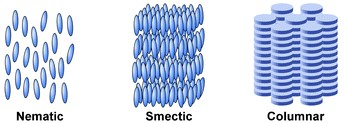
\includegraphics[width=0.7\linewidth]{Figures/lc_phases_cropped}
	\caption{Representation of the three liquid crystal phase classes, reproduced from Kato et al. \cite{Kato2007} with permission. Note the distinct layers in the smectic and columnar phases, and the different class of molecule in the columnar phase.}
	\label{fig:lcphasescropped}
\end{figure}


It should be noted that the higher order phases (smectic and columnar) also display orientational order throughout the body. This is fundamental to the formation of liquid crystals, and so (almost) all mesogenic molecules are anisotropic. We will see later that the degree of anisotropy affects the stability of different phases. 

As is visible in Figure \ref{fig:lcphasescropped}, this anisotropy can come in different forms. `Rod-like' molecules (where anisotropy is in the form of one elongated axis) are the oldest, and most popular, form of liquid crystal. They favour the formation of nematic and smectic phases, and will form the focus of this report. Alternatively, disk shaped (discotic) molecules (discovered by Chandrasekhar in 1977 \cite{Chandrasekhar1977}) have one compressed axis, and favour the formation of other nematic or columnar phases. In 1987, Lam subsequently predicted the existence of a sub-class of `bowlic' molecules which break the up-down symmetry of discotic molecules \cite{LinLei1988}, which were subsequently found experimentally \cite{Zimmermann1985, Malthete1985}.

Liquid crystals can also be categorised by the driving force behind the transition. Smaller molecules tend to undergo thermally driven phase transitions, and so form different thermotropic phases in different temperature ranges. By contrast, larger molecules tend to undergo lyotropic, or concentration driven phase transitions \cite{DeGennes1993}. The focus of this report will lie in such phase transitions, and specifically in entropically driven phase transitions where the interaction potentials are purely repulsive. These are an effective benchmark for DNA\textendash-based systems; where Debye screening means the potential is almost purely repulsive

Entropically driven are often seen as counter-intuitive, as such transitions rely on an increase in microscopic disorder from a increase in visible order (an example of this is given in Section \ref{sec:OnsagerTheory}). Once considered an abnormality, Frenkel famously noted that ``\textit{...such phase transformations may not be interesting exceptions, but the rule!}'' \cite{Frenkel1999}.

\subsection{Onsager Theory} \label{sec:OnsagerTheory}

Onsager predicted a simple model of lyotropic, entropy-driven phase transitions \cite{Onsager1949}, which will be employed in this project. Rod-like particles are modelled as thin spherocylinders with length $L$ and diamater $D$, and an excluded volume preventing overlap. The interaction potentials between molecules are neglected, and only the configurational entropy of the system considered. Qualitatively, the confinement of rods to parallel orientations (such as in the nematic phase) leads to a decrease in orientational entropy, but an increase in positional entropy (as each rod takes up less space). At sufficiently high concentrations, the positional entropy will dominate, and the system undergo a phase transition from isotropic to nematic. 

The critical volume fraction at transition is approximately $4r/L$, where $r$ is the radius of the rigid rod, and $L$ is the length (detailed of this are given in Appendix \ref{sec:OnsagerAppendix}. Crucially, this means the isotropic--nematic phase transition occurs at lower concentrations for mesogens with greater aspect ratios, and requires a minimum aspect ratio of $L/r = 4$ to occur. It is worth noting that this result is only valid in the limit of thin spherocylinders, as Onsager's derivation neglects Virial coeffecients $B_{n}$ beyond second order in the expansion of free energy in powers of density \cite{Frenkel1987}; further discussion of this is given in Appendix \ref{sec:OnsagerAppendix}. Despite this, Onsager's theory has since been well tested, with both computational \cite{Frenkel1987b, Frenkel1988b} and experimental \cite{Kubo1979,Oldenbourg1988,Fraden1993} results substantiating its validity.

%penultimate sentence could go into appendix
% validation of Onsagers theory in https://doi-org.ezp.lib.cam.ac.uk/10.1021/ar9500224
% also backed up in simulation context at start of rigid rods section


\subsection{Order Parameter}
%smectic order given by frenkel https://pubs.acs.org/doi/pdf/10.1021/j100322a042
%can also use https://www.tandfonline.com/doi/full/10.1080/00268976.2018.1471231

The degree of order in a liquid crystal phase is characterised by an order parameter, chosen such that it is non zero in the ordered phase but vanishes in the isotropic phase. A familiar example of this is the magnetisation $\textbf{M}$ of a ferromagnet; when raised above a critical temperature, the magnetisation vanishes as the ferromagnet undergoes a phase transition. While the choice of order parameter for the nematic phase transition is less intuitive than this, it relies on the formation of genuine long-range orientational order. We may therefore define the angle ($\theta$) between each molecule's axis and the system director, and traditionally let the order parameter S be given by:

\begin{equation}
S_{n} = \left\langle P_{2}(\cos(\theta)) \right\rangle = \left\langle \frac{3}{2}\cos^{2}(\theta) - \frac{1}{2} \right\rangle 
\end{equation}

where $P_{2}$ simply denotes the second Legendre polynomial \cite{DeGennes1993}. While $\langle \cos^{2}(\theta) \rangle$ would function alone as the order parameter, this has the useful property of giving unity for a perfectly aligned system, and zero for a completely random system. Further motivation for this choice is provided in Appendix \ref{sec:OrderParamTheory}.

%add description of pair-wise orientational order coeff

Similarly we will find it helpful to define a smectic order parameter $S_{s}$, to characterise the formation of one-dimensional long-range positional order. Intuitively, we expect a non-zero Fourier component of the normalised density along the director \cite{Polson1997}, and so we may write:

\begin{equation}
S_{s} = \frac{1}{N} \left\lvert \sum_{j=1}^{N} \exp \left( {\frac{2\pi}{L}i\textbf{r}_{j} \cdot \boldsymbol{\hat{n}}} \right) \right\rvert
\end{equation}

for a layers of periodicity $L$ perpendicular to the nematic director $\boldsymbol{\hat{n}}$, and where $\textbf{r}_{j}$ denotes the centre of mass position of the $j$th molecule \cite{Dussi2018}.


\subsection{DNA as a Liquid Crystal} 
%zhao2019 is useful review and gives onsager theory
%nakata is beyond onsager theory
%wang2018 gives useful section on history
Lyotropic liquid-crystalline phases are very common in living systems, from cellular membranes to fibroblast structures \cite{Stewart1966, Rey2013}. In vitro, many biochemical molecules such as cellulose, peptides, and protein assemblies have also been shown to form liquid crystal states \cite{Zhao2019}. With respect to the mesogenic behaviour of DNA, Luzzati et al. first observed a columnar phase in a condensed DNA solution in 1959 (only 6 years after the discovery of the double-helix structure), and Robinson pioneered the development of the twisted-nematic phase in 1961 \cite{Luzzati1959, Robinson1961}. Subsequent work by Strzelecka et al. has demonstrated experimentally that DNA molecules can form precholestric, cholestric and smectic phases (in order of increasing concentration) though lyotropic phase transitions \cite{Strzelecka1988}. 

Returning to Onsager's theory, with the known dimensions of DNA we find that that the minimum base pair length required to obtain liquid crystalline phase behaviour is 24 base pairs \cite{Bolhuis1997}. However this limit has been broken experimentally by Nakata et al. \cite{Nakata2007, Zanchetta2008}, which they suggest is a result of monomer stacking through end-to-end adhesion to form the larger mesogens required.

These techniques may be applied to developing DNA origami, the process whereby complex nano-structures are constructed out of DNA molecules. Though a greater understanding of the phase behaviour of DNA nanoparticles, we may inform design of more complex structures, and develop colloidal self-assembly processes. These techniques may have applications in fields as diverse as biophysics, photonics, structural biology, and synthetic biology \cite{Nummelin2018, Praetorius2017, Bathe2017}.

%mention debye screening length argument, and how purely repulsive potentials are both useful and accurate

\subsection{Previous Simulation Work} \label{sec:PrevWork}
Computational work may be implemented over a broad spectrum of coarse-graining (a process whereby microscopic degrees of freedom are integrated over to reduce the computational costs of a simulation at the cost of lower model resolution), where the base unit of the simulation ranges from single atoms to large bulk molecules \cite{Inglfsson2013, Potoyan2012}. Atomistic models, such as CHARMM \cite{MacKerell1995} and AMBER \cite{SalomonFerrer2012}, offer the greater level of detail, but are limited by computational cost beyond small (>30 base pairs) models \cite{Cheatham2004}. In contrast, bead-spring polymer models (with up to 3000 base pairs per bead) may obtain bulk material properties at significantly lower computational expense \cite{Michieletto2016}.

Such models have been applied specifically to DNA nunchucks by Salamonczyk et al. \cite{Salamonczyk2016} to suggest the existence of smectic phases, however this is limited by the level of coarse-graining applied, as the artificial interaction potentials considered have no physical origin. This project work builds on this research, by applying a intra-molecular potential derived by single nucleotide simulations of the nunchuck molecule by Jiaming Yu (within the Eiser Group) using OxDNA, a lower-level coarse grained model that accurately represents the physical properties of single and double stranded DNA \cite{OxDNA}.

My work is based on a coarse-grained model developed by Xing et al. \cite{Xing2019} to consider Y-shaped nanoparticles constructed from DNA, and utilises LAMMPS \cite{LAMMPS} software to model dense systems of these nunchuck nano-particles. This approach applies the increased resolution of the single nucleotide OxDNA model to larger systems of many such molecules, to provide a better predictor of this system's experimental phase behaviour.

\section{Methods} \label{sec:Methods}
As introduced in Section \ref{sec:PrevWork}, all molecular dynamics simulations were completed in LAMMPS. LAMMPS (Large-scale Atomic/Molecular Massively Parallel Simulator) is a medium coarse-grained, classical molecular dynamics code developed to replicate  solid-state materials and soft matter mesoscopic systems \cite{Plimpton1995, LAMMPS}.


%Can expand on this if needs be, from rapaport

\subsection{Simulation Molecules} \label{sec:SimMolecules}
As introduced in Section \textbf{X}, we are considering `nunchuck' molecules formed of two rigid rods connected by a flexible linker, as depicted in Figure \ref{fig:nunchuck_analogy}. However, as the interaction potential of an anisotropic particle is rather complex, it is computationally simpler to consider each molecule as a system of connected spheres, each with a separate isotropic interaction potential (detailed further in Section \ref{pair_potential}).

This is visualised in Figure \ref{fig:nunchuck_implementation}, for rigid arms of aspect ratio 7. The ss-DNA is represented by a further sphere in the centre of the molecule, coloured differently in red to highlight its differing mechanical properties. It has a modified bond angle, so the molecule is bent around this element, and reduced bond rigidity so the particle may also stretch about this point. We also consider a simplified system of rigid rods with no modifications on the central atom, to verify the analysis methods against known results.

\begin{figure}[ht]
	\hfill  %NOT SURE ABOUT THIS!
	\begin{subfigure}{.4\textwidth}
		\centering
		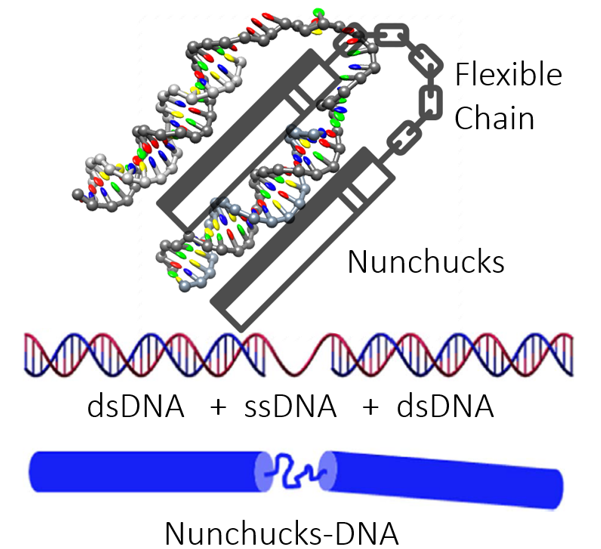
\includegraphics[width=\linewidth]{Figures/nunchucks_artist}  
		\caption{Coarse-grained Model}
		\label{fig:nunchuck_analogy}
	\end{subfigure}
	\hfill %% useful if width of each figure is less the .5\textwidth
	\begin{subfigure}{.4\textwidth}
		\centering
		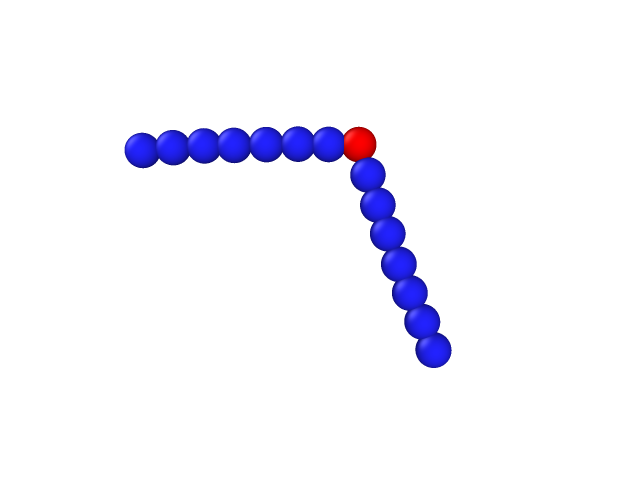
\includegraphics[width=\linewidth]{Figures/nunchuck_profile_coloured}  
		\caption{LAMMPS Implementation}
		\label{fig:nunchuck_implementation}
	\end{subfigure}
	\caption{Depiction analogy between the DNA mesogen and the nunchucks. Note the appearance of the flexible ss-DNA linker between the rigid ds-DNA rods, and the implementation within LAMMPS on the right. The central red sphere, representing the ss-DNA, is given modified bond properties to replicate the nunchuck's flexibility. Figure (a) created by Jiaming Yu (Eiser Group, Cambridge).}
	\label{fig:nunchucks_visual}
	\hfill
\end{figure}

A system of natural units was used in simulations, and replicated in our results here. Based on the Lennard-Jones potential, the cut-off length and characteristic energy are both set to unity. The simulation timescale is then fixed by the choice of these values, and the mass of the simulation body. 

The physical values for a system may be considered for a specific system (in this case strands of ds-DNA) through scaling via the relevant mass, length scale and energy scale of this system. However the dimensionless simulations presented here may be generalised to any similarly-shaped mesogens; we would expect other systems to display the same behaviour over an appropriate timescale determined by their material properties \cite{Rapaport2004}.

For the nunchuck particles considered, a length scale of \SI{2}{\nano\metre} is used (corresponding to the width of ds-DNA, and hence the diameter of a simulation sphere) \cite{Arnott1972}. It is worth noting that the persistence length of DNA is around \SI{50}{\nano\metre} \cite{Garcia2007}, so the approximation of perfect rigidity is valid for all rods considered here (maximum length \SI{30}{\nano\metre}). Using the standard value of \SI{0.33}{\nano\metre} \cite{Langridge1960} for the average length of a base pair, each sphere corresponds to a sequence of six base pairs. This gives the mass of each sphere as \SI{6.5e-24}{\kilogram}, based on an average formula mass per base pair of \SI{650}{\dalton} \cite{Duewer2018}). 

We may also define the characteristic energy scale; this is formally the depth of the potential well in the full Lennard-Jones potential, but the thermal energy serves as a common approximation \cite{Pan2010} in agreement with experimental data \cite{Wang2002}. Using these values, we find that the characteristic timescale for this system is \SI{79}{\pico\second}. In this context, the simulation timestep would be \SI{0.4}{\pico\second}, and typical simulation of \num{20e6} steps had a total duration of \SI{7.9}{\micro\second}. For \num{1000} particles, this took approximately $8$ hours to run on a standard laptop CPU. %check these



\subsection{Simulation Structure} %was? is? check your tense here!
All simulations in this report were conducted a system of 1000 particles, with a time step of $0.005\tau$, (where $\tau$ is the characteristic time), unless otherwise stated. The system was initially configured in a dilute, isotropic state; a non-trivial process for large numbers of mesogens as molecules must be placed randomly without overlap, to prevent any initial order affecting the formation of ordered phases. I am grateful to Iria Pantazi for writing a python script to automate this process for dilute rigid rod systems, and a generalised version of this is available in the supplementary material. Alternatively, simulations were also initiated from a perfectly ordered square crystalline phase, with all molecules aligned along a common axis. The choice of this axis is arbitrary, as the system is invariant under global rotation \cite{Nos1983}, but is taken to be directed along the y-axis for clarity. Care was taken to ensure molecules did not overlap, and the system was stable in this ordered phase.
%MAYBE INCLUDE CODE IN SUPP MATERIAL?? THINK ABOUT THIS!

All simulations are conducted within an oblong box defined by the Cartesian axes, with periodic boundary conditions used to eliminate surface effects and replicate conditions in the bulk phase \cite{Frenkel2002}. The aspect ratio of this box may be varied, to support phase formation in anisotropic systems, as discussed in Section \textbf{X}. An isenthalpic ensemble was used (where pressure is fixed) to vary the size of the simulation region (either contracting or expanding), allowing sampling of different volume fractions from the same initial configuration. The microcanonical ensemble, where both the system volume and energy are conserved, was then used to allow the system to reach thermodynamic equilibrium. Time integration was evaluated using the Nose-Hoover thermostat \cite{Nos1984, Hoover1985} natively implemented in LAMMPS \cite{Shinoda2004}, typically with a damping time of $\tau$.

A typical simulation consists of multiple stages, alternating between these two ensembles to sample the system properties at a range of volume fractions. Approximately \num{2e4} steps are simulated when varying the simulation volume (depending on the resolution of volume fraction sampling), followed by \num{2e6} to allow the system to reach equilibrium in each stage. The output of thermodynamic variables, as well as particle positions, at the end of each stage allows for subsequent calculation of the order parameter at equilibrium. This data was also retrieved at regular intervals during each simulation stage, to track the time evolution of the system.

To ensure stability of the system, a Langevin thermostat \cite{Schneider1978} was also used throughout, and energy conservation was verified over a range of timescales. The damping for all thermostats is equal to the characteristic timescale of the simulation (i.e. unity in natural units).



\subsection{Intermolecular Potential} \label{pair_potential}
A shifted, cut-off Lennard-Jones potential was chosen to represent pair-wise interactions between molecules. While the Lennard-Jones potential \cite{Jones1924a, Jones1924b} has long been the natural choice for molecular dynamics simulations \cite{Stephan2019}, its infinite range introduces computational complexity as interactions between all pairs of particles must be considered. It is therefore increasingly common to use a cut-off version, whereby the potential is set to zero beyond a `cut-off' radius, and here we chose to neglect the entire attractive tail. As well as simplifying the calculations required, this also allows our results to be generalised to any mesogens without attractive inter-molecular forces (that typically favour ordered-phase formation), as any phase transitions observed here must be purely entropically driven. This is commonly known as a soft-core model, where particle overlap is suppressed via this repulsive potential rather than any excluded volume interactions, and is computationally much less demanding \cite{Paolini1993, Hughes2008}.
%can cite frenkel on entropically drive transitions if req

However, this cut-off may cause unphysical behaviour if the potential does not tend to zero smoothly at this point. This is remedied by the addition of a constant term, described in the full form of the pair-wise potential $U_{ij}$ in (\ref{lj_cut}):

\begin{equation} \label{lj_cut}
U_{ij} = 4\epsilon \left[ \left( \frac{\sigma}{r_{ij}} \right) ^{12} - \left( \frac{\sigma}{r_{ij}} \right) ^{6}	\right] + \epsilon \qquad	 r_{ij} < r_{c} = 2^{1/6} \sigma
\end{equation}

Here $\sigma$ and $\epsilon$ are the relevant length and energy scales of the system, formally corresponding to the particle separation at which the $U_{ij} = 0$, and the depth of the potential well. It is worth noting that the effects of this truncation and shift on the overall thermodynamic quantities are well documented \cite{Stephan2020, Shaul2010}, and changes in lyotropic properties are negligible in 3D bulk liquids with a conserved particle number \cite{Smit1991}. This purely repulsive potential is also a good representation of the physical DNA system considered here, for appropriate salt concentration in the solvent \cite{Strey1997, Strey1998}.

 
\subsection{Analysis Methods}
The visualisation freeware Ovito \cite{Ovito} has been employed to animate the molecule motion over the simulation period, and was used to generate all molecular images presented here. Thermodynamic variables, such as internal energy and pressure, were extracted to track the system's progress towards equilibrium, and verify its stability.

The volume fraction and nematic order parameter were computed for comparison with Onsager's theorem, as detailed in Section \ref{sec:OnsagerTheory}. Calculation of the order parameter is complicated by the absence of an imposed director (ie if no electric field is applied), and we use the approach taken by Eppenga and Frenkel \cite{Eppenga1984} which is reproduced in Appendix \ref{sec:OrderParamCalc}. %or dussi 2018 or many others

Further analysis included the calculation of the smectic order parameter, and pair-wise orientational correlation coefficient, detailed in Section \textbf{X}. All scripts for data extraction and analysis were written by the author, \textit{and can be found in the supplementary material?}.



\section{Rigid Rod Simulations} \label{sec:RigidRodSims}
%Used to benchmark sys etc and demonstrate techniques to identify phase transitions.
%Detail nematic phase transition (longrun4) and validation through onsager theory
%Extend this with the longer rods which continue to confirm this theory


Initially, a system of rigid rods was used to verify the analysis methods applied in this report, in comparison with the predictions made by Onsager's theory in Section \ref{sec:OnsagerTheory}. We focus specifically on the phase transition between the isotropic and nematic phases, as this system is well studied, and these predictions have been separately verified computationally through both Monte Carlo \cite{Frenkel1984, Lee1987} and molecular dynamics simulations \cite{Allen1987, Camp1996}.
%not experimentally; long-range maier-snape is better here https://pubs.acs.org/doi/pdf/10.1021/j100303a008

\subsection{Contracting Simulations}

For rigid rods with an aspect ratio $L/D = 10$, Onsager theory predicts a lyotropic phase transition will occur, with a critical volume fraction of $\phi  = 0.4$. We consider a system of \num{1000} rigid rods, formed of \num{10} sequentially connected `balls' (force-centres), and apply alternating stages of contraction (where the volume fraction is increased) and equilibration (where the volume is held constant). Each contraction stage consists of between \num{1e4} and \num{5e4} steps (chosen to identify the critical volume fraction with maximal resolution, while verifying the order parameter is approximately constant outside of this), while the equilibration stage runs for \num{2e6} steps. In this way we are able to confine the possible critical volume fraction to the range $0.39 < \phi< 0.44$, as observed in Figure \ref{fig:rr_nemorderparam}, in good agreement with Onsager's prediction of $\phi = 0.4$.

\begin{figure} [h!]
	\centering
	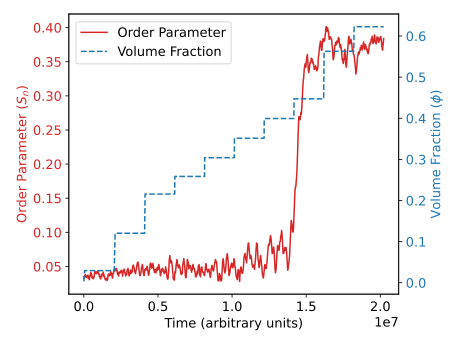
\includegraphics[width=0.7\linewidth]{Figures/rigidrod_nemorderparam}
	\caption{The evolution of the volume fraction ($\phi$) and the nematic order parameter ($S_{n}$) over the timescale of the simulation, for a system of 1000 rigid rods with aspect ratio 10. The phase transition is observed through a discrete change in the order parameter (in red), occurring after the volume fraction is increased above $0.4$. Note that the contraction steps (where volume fraction is changed) are not of equal durations, and so do not correspond to equal changes in the system volume; rather they are chosen to highlight the phase transition. The timescale of contraction is much less that the timescale of equilibration, but the changes in volume fraction are not instantaneous, despite their appearance here.}
	\label{fig:rr_nemorderparam}
\end{figure}  %C:\Users\KitG\Documents\LC_Project\Phase_Structure\Rigid_Rods2

This analysis was then repeated with longer rods, having an aspect ratio of \num{16} and a predicted critical volume fraction of $\phi  = 0.25$. Through multiple simulations, we are similarly able to verify that the critical volume fraction lies in the range $0.23 < \phi< 0.26$, in good agreement with the theory. This also provides a useful example of the characterisation of a phase transition through changes in the thermodynamic variables; Figure \ref{fig:rr_pressureevo} depicts a change in pressure during the equilibration stage of the simulation (during which volume is conserved) corresponding to the isotropic\textendash nematic phase transition.

\begin{figure} [h!]
	\centering
	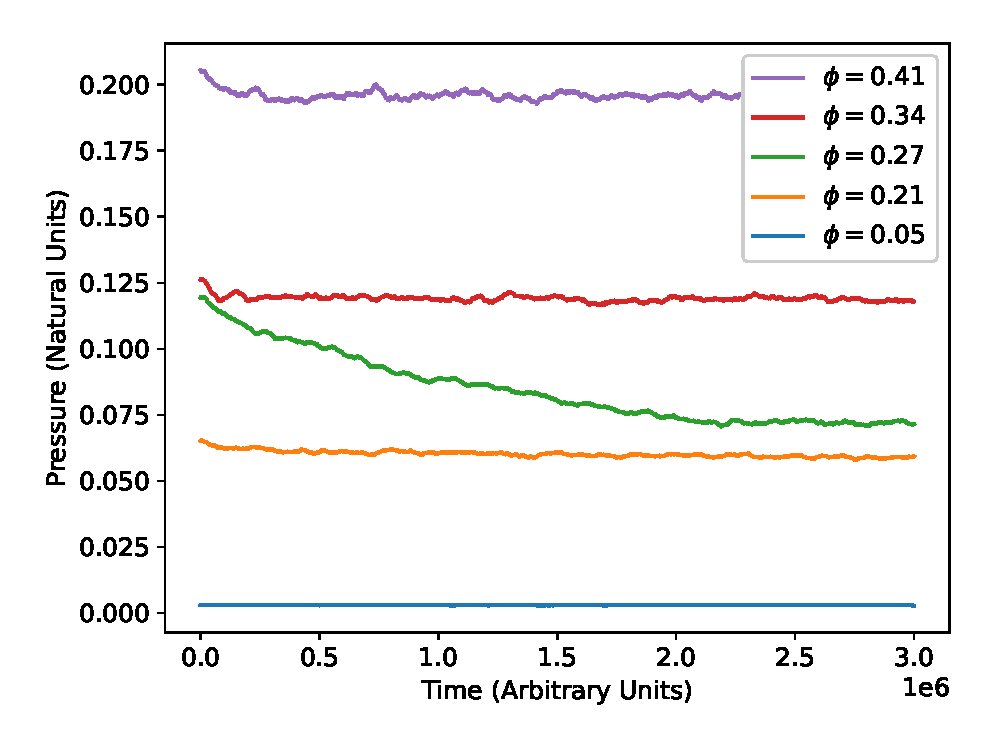
\includegraphics[width=0.7\linewidth]{Figures/rigidrod_pressureevo}
	\caption{The evolution of pressure on subsequent microcanonical ensembles (between which volume is decreased), when simulating 1000 rigid rods of aspect ratio 16. Note the extended decay in pressure for $\phi  = 0.27$, while the isotropic\textendash nematic phase transition occurs; all other stages remain at equilibrium throughout.}
	\label{fig:rr_pressureevo}
\end{figure} %C:\Users\KitG\Documents\LC_Project\Phase_Structure\Rigid_Rods2\Double_Length_Rods



\subsection{Expanding Simulations}
%Explain motivation for running simulation in reverse
%Validate location of nematic phase transition
%Introduce additional smectic phase transition (is there literature on the predicted volume fraction here?)
%explain uncertainty on nature of nematic-> smectic transition

We may also consider phase behaviour upon expansion from an perfectly ordered state, in hope of observing the same phase behaviour `in reverse'. This has two advantages; it allows us to access higher volume fractions that are not easily accessible through molecular dynamics simulations (of a reasonable duration), and also provides verification of the phase transitions previously observed. Ensuring a novel phase is in true equilibrium has long been the bane of liquid crystal simulators, however non-equilibrium effects will manifest themselves in hysteresis of the phase transition (variation in the critical volume fraction dependant on the direction of the transition), and so can be easily identified through this method.

Initially, the particle force centres are configured in a simple cubic crystalline lattice. Again equilibration stages under the microcanonical ensemble (with constant volume) are ran in alternation with an isenthalpic ensemble, however the target pressure for the Nose-Hoover thermostat is now reduced below the system pressure so that expansion occurs in these isenthalpic stages. The length of these stages is unchanged from Section \ref{sec:RigidRodSims}, however the thermostat damping is increased to $100\tau$ to ensure stability of the expansion.

\begin{figure} [h!]
	\centering
	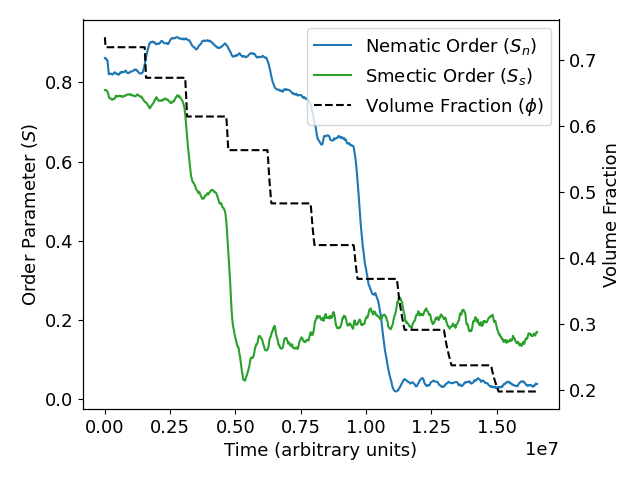
\includegraphics[width=0.7\linewidth]{Figures/rigidrod_cryorderparam}
	\caption{The evolution of the volume fraction ($\phi$) against both the nematic ($S_{n}$) and smectic ($S_{s}$) order parameters over the timescale of the simulation, for a system of 1000 rigid rods with aspect ratio 10 initiated in a crystalline phase. A continuous smectic\textendash nematic phase transition is observed (in green) at high volume fractions, followed by a discrete nematic\textendash isotropic transition (in blue), occurring after the volume fraction is decreased below $0.4$. Note that there are multiple steps in the smectic order parameter, indicating this transition occurs over a range of volume fractions.}
	\label{fig:rr_crystalorder}
\end{figure} %C:\Users\KitG\Documents\LC_Project\Phase_Structure\Rigid_Rods2\Crystalline\Full_Transition


The isotropic phase formation was observed in the region $0.38 < \phi< 0.41$, in good agreement with the results of Section \ref{sec:RigidRodSims}, and confirming this is indeed an equilibrium phase transition. 

The higher volume fractions accessed at the start of the simulation also give rise to another phase transition; forming this nematic phase from the initial ordered phase. While the system was configured in a crystalline phase, it quickly relaxes into an smectic-like phase with the one-dimensional long-range positional order. The subsequent smectic\textendash nematic transition is then observed in Figure \ref{fig:rr_crystalorder}, with a reduction in the smectic order parameter around $\phi  = 0.6$. This transition is clearly concentration-dependant (with discrete jumps in the order parameter when the volume fraction is reduced), however it occurs over a range of volume fractions and so is likely a continuous phase transition. While our evidence here is not conclusive, this is still a matter of active research and beyond the scope of this report. Theoretical \cite{Wen1987}, computational \cite{Frenkel1988, McGrother1996}, and experimental \cite{Dogic1997, Doane1972} evidence however suggests that this transition is expected to be continuous (or at most weakly first-order) for rigid rods of extended aspect ratios, and occur around this volume fraction. 
%Frenkels results also find no dependance on aspect ratio (for crit volume frac)
%Later suggested that this transition is only continuous at large aspect ratios, and first order for ratios much smaller than are used here.
%Dogic suggests continuous for rigid particles, but first order if flexible, Doane uses hydrocarbon chains to come to the same conclusions

\section{Nunchuck Simulations} \label{sec:Nunchuck_Sim}
Further simulations applied the same approaches to the nunchuck molecules introduced in Section \ref{sec:SimMolecules}. These could be configured in two ways; either with a fixed angle between the two rigid arms, or a fixed rigidity (which determines the angular potential between the two arms, and hence the distribution of angles observed). Previous work by Jiaming Yu using OxDNA \cite{OxDNA} has suggested that the fixed rigidity model provides an accurate coarse-grained model of the nunchucks; however the fixed angle approach is also used for simplicity, and because it appears more amenable to ordered phase formation.

describe the challenges in phase identification here, with references if possible

%different phases possible https://pubs.rsc.org/en/content/articlelanding/2011/SM/c1sm05751k#!divAbstract
%biaxial neamtics (feroomagnetic) https://pubs.acs.org/doi/pdf/10.1021/cm980631g
%dimers with central flexible spacer https://pubs.rsc.org/en/content/articlepdf/2014/tc/c4tc00212a

\subsection{Fixed Rigidity}
%basic formation of nematic-like phase
%change in angle distribution to generate order 

Initially, the fixed rigidity case is considered, with a rigidity parameter of \num{0.1}, giving complete bond flexibility. Despite this, a nematic-like phase was formed at volume fractions $\phi > 0.4$, although with a maximal order parameter of \num{0.25} significantly below that observed previously in nematic phases, indicating that this was not truly nematic. This quasi-ordered phase can be observed in Figure \ref{fig:nun_fr_views}, where clear short range orientational order is visible, but the preferential orientation varies across the simulation region.

\begin{figure}
	\centering
	\begin{subfigure}{.5\textwidth}
		\centering
		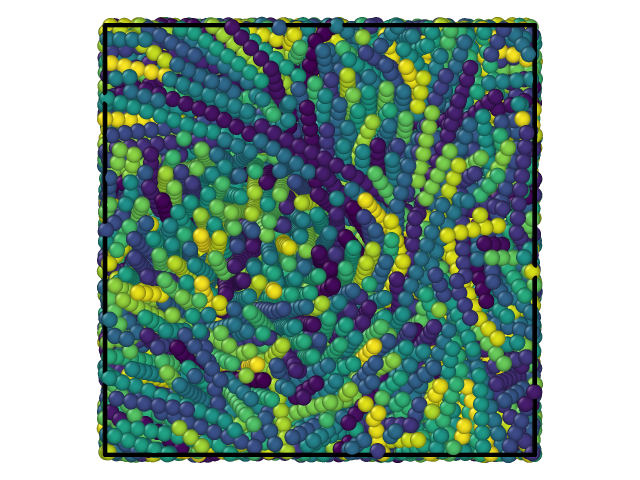
\includegraphics[width=.9\linewidth]{Figures/nun_fr_side}
		\caption{Side View}
		\label{fig:nun_fr_side}
	\end{subfigure}%
	\begin{subfigure}{.5\textwidth}
		\centering
		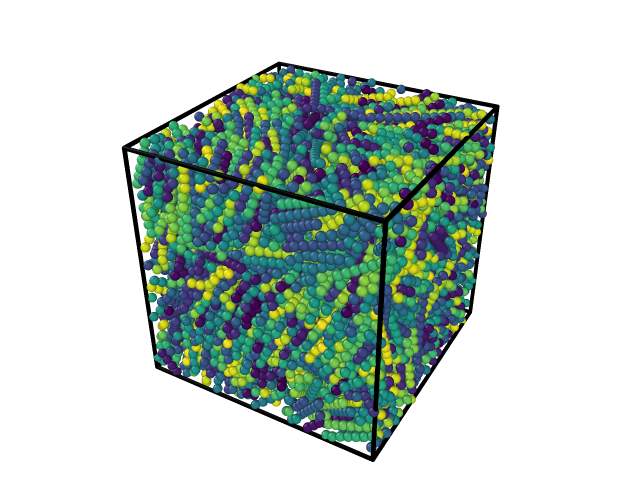
\includegraphics[width=.9\linewidth]{Figures/nun_fr_perspective}
		\caption{Perspective View}
		\label{fig:nun_fr_perspective}
	\end{subfigure}
	\caption{The quasi-ordered phase formed by \num{1000} fully flexible nunchucks. Note the local regions of aligned rods, suggesting a nematic-like phase, but also the variation of the director across the sample (between these regions). The length scale of any periodicity in this variation is larger than the simulation box itself.}
	\label{fig:nun_fr_views}
\end{figure} %C:\Users\KitG\Documents\LC_Project\Phase_Structure\Nunchucks\Fixed_Rigidity\stretch500_rigidity5_len15

\begin{figure} [h!]
	\centering
	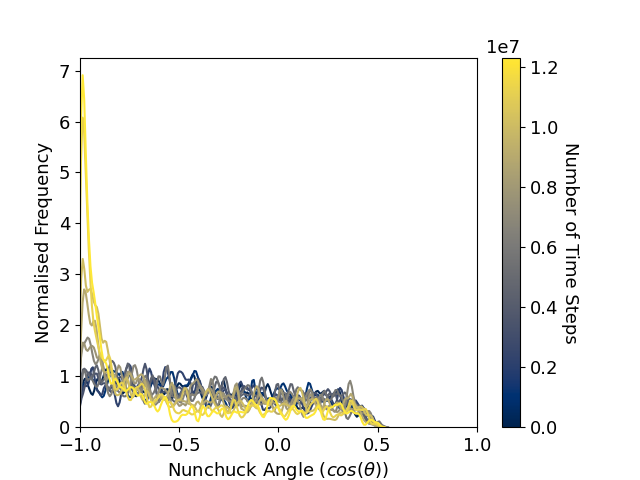
\includegraphics[width=0.7\linewidth]{Figures/nun_fr_angledist}
	\caption{A kernel density estimate plot of the distribution of nunchuck opening angle (between the two rigid arms) over time (as the volume fraction is reduced), where nunchucks are completely flexible. Plotted for a system of \num{1000} particles, with the distribution sampled every \num{1e6} time steps. Note the formation of a preferential angle at late times, corresponding to the formation of an ordered phase at high volume fractions.}
	\label{fig:nun_fr_angledist}
\end{figure}  %C:\Users\KitG\Documents\LC_Project\Phase_Structure\Nunchucks\Fixed_Rigidity 

Consideration of the distribution of nunchuck bond angles (i.e. the opening angle between the two rigid arms) gives further evidence for some ordered phase formation however, with a clear preferential angle forming in Figure \ref{fig:nun_fr_angledist}. We suggest that the length scale over which this director varies is greater than the size of the simulation region, preventing use of the orientational correlation function described in Section \textbf{X} as well. Unfortunately the computational resources required to simulate larger systems was beyond the scope of this project, due to the scaling of the number of particles required to achieve the same volume fractions. 



\subsection{Fixed Angle}
We therefore transfer our focus to systems where the nunchuck opening angle is confined to a particular value, as we suggest similarly quasi-nematic structures may be observed on shorter length scales,  particularly this opening angle is confined below the mean angle of Figure \ref{fig:nun_fr_angledist}.
We tested phase formation over a range of rigid rod lengths and opening angle values; broadly we found that larger opening angles favoured nematic-like phase formation (which our analysis methods were best suited to identify), but smaller angles did not form obvious alternate ordered phases. An example of the phases formed if given in Figure \ref{fig:nun_fa_views}, which depicts a quasi-nematic structure.

\begin{figure}
	\centering
	\begin{subfigure}{.5\textwidth}
		\centering
		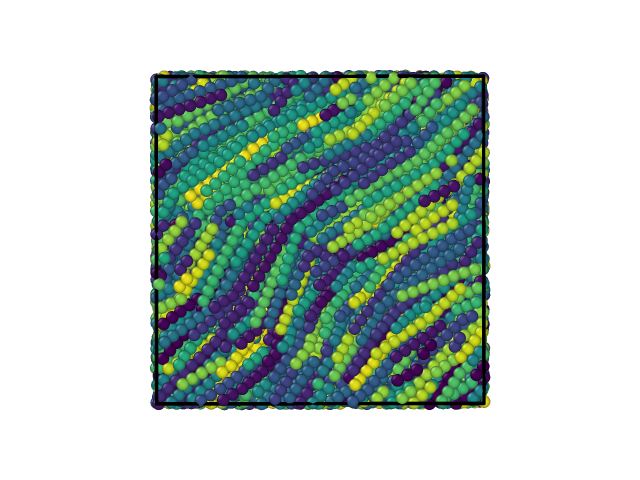
\includegraphics[width=.9\linewidth]{Figures/nun_fa_side}
		\caption{Side View}
		\label{fig:nun_fa_side}
	\end{subfigure}%
	\begin{subfigure}{.5\textwidth}
		\centering
		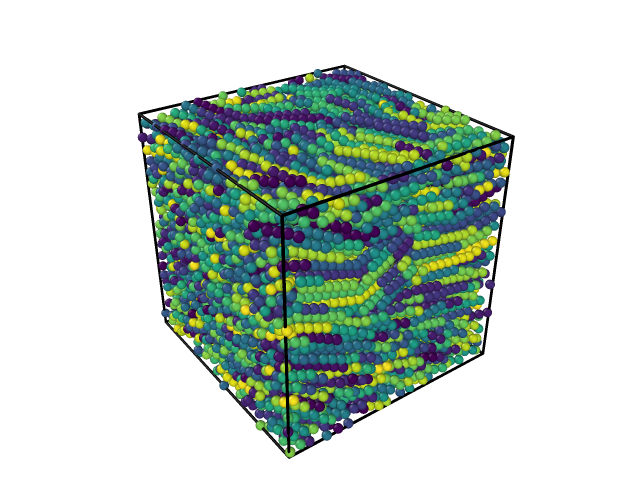
\includegraphics[width=.9\linewidth]{Figures/nun_fa_perspective}
		\caption{Perspective View}
		\label{fig:nun_fa_perspective}
	\end{subfigure}
	\caption{The quasi-ordered phase formed by \num{1000} nunchucks with an opening angle of \SI{150}{\deg}. Note the global alignment of molecule directors, giving a high nematic order parameter, but also the alternating herringbone-like structure.}
	\label{fig:nun_fa_views}
\end{figure}

Alongside the nematic tendency here for all molecules to have similar alignment along a constant global director, there appears to be more periodic ordering, such as the herringbone structure clearly visible in Figure \ref{fig:nun_fa_side}. This cannot be described by our current order parameter methods, and a different method is required.


\subsection{Orientational Order Parameter} \label{sec:PairWise_Application}
The suggestion of novel phases in these systems first requires alternative methods to characterise the order of the system; this are typically motivated by the class of symmetry expected here. Given that our system appears to display a degree of orientational order, a length-dependant orientational order parameter is introduced to verify this order is indeed long-ranged (and not simply due to short range steric effects). This also allows the identification of any periodic aspects to the system, as the bend in the nunchucks might be expected to result in the formation of a twisted nematic phase; these would be observed as oscillatory components in the order parameter.

We consider an $l$-th rank pair-wise correlation function, where $g_{l}(r)$ gives the correlation between the orientation of two particles separated by a distance $r$ :

\begin{equation} \label{eq:PairWise_eq}
g_{l}(r) = \frac{\langle P_{l}(\boldsymbol{\hat{u}_{i}}\cdot \boldsymbol{\hat{u}_{j}}) \delta(r_{ij}-r)\rangle}{\langle  \delta(r_{ij}-r) \rangle}
\end{equation}

where $\boldsymbol{\hat{u}_{i}}$ is the director for molecule $i$, and $r_{ij}$ is the separation between a given pair of molecules $i,j$ \cite{Zannoni1979}. In the disordered phase, this decays to zero, while in the ordered phase it decays to the square of the orientational order parameter \cite{Frenkel1985b}:

\begin{equation}
\lim_{r \to \infty}g_{l}(r) = \left\langle P_{l} \right\rangle ^{2}
\end{equation}

Details of the calculation methods of $g_{l}(r)$ are given in Appendix \ref{sec:PairWise_Theory}. 

This may be applied to the system observed in Figure \ref{fig:nun_fa_views}, however this approach is limited by the length scale of the simulation region; the maximum separation between particles is half the size of the simulation region due to the periodic boundary conditions \cite{Frenkel1985c}.

To determine order over longer length scales, without increasing the volume of the system (due to the limited computational resources), we instead vary the aspect ratio of the system. By considering instead an elongated oblong simulation region, we are able to sample correlations over longer distances (along the long axis of the box) for systems of the same particle number. As depicted in Figure \ref{fig:num_fa_correlation_mol}, this method gives conformation that the order observed in this fixed angle system is indeed long-range, and does not decay at long length scales.

\begin{figure} [h!]
	\centering
	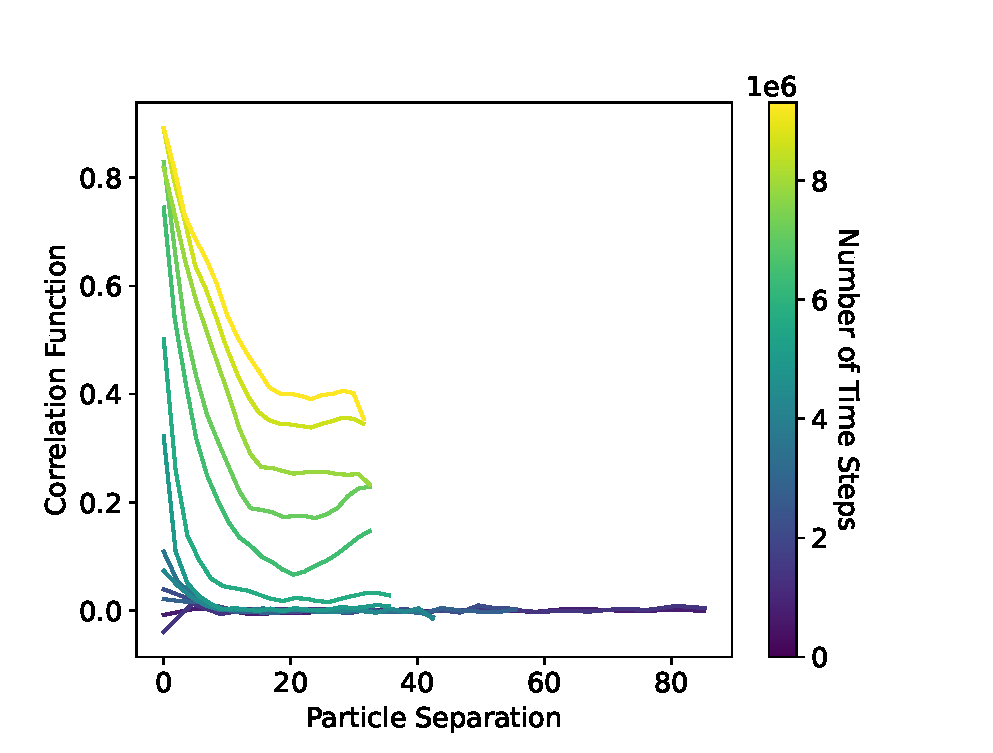
\includegraphics[width=0.7\linewidth]{Figures/num_fa_correlation_mol}
	\caption{Orientational correlation function over time (as the volume fraction is reduced), where nunchucks have a fixed opening angle (between the rigid arms). Plotted for a system of \num{1000} nunchuck molecules, with an opening angle of \SI{150}{\deg}, being sampled every \num{7e5} time steps. Note the formation of an ordered phase at high volume fractions (late times), with sustained long-range order (i.e. no decay in the orientational correlation function). The maximum value of particle separation (in arbitrary length units) is determined by the size of the simulation box, and so shrinks over time. }
	\label{fig:num_fa_correlation_mol}
\end{figure}  %C:\Users\KitG\Documents\LC_Project\Phase_Structure\Nunchucks\Fixed_Angle\2_bend_165_deg_oblong


This method is however fundamentally limited by the use of a single vector along the molecular axis to define the orientation of the molecule; two vectors (such as along each arm) are required to uniquely specify the orientation of a single molecule. Using the molecule axis alone only accounts for quasi-nematic order; any biaxial or herringbone substructure must be accounted for differently. We therefore also consider orientational correlation functions for the vectors along the bisector of each molecule, and normal to the plane of the nunchuck. It is worth nothing that the second Legendre polynomial is still used when taking the normal vector, however the first Legendre polynomial is used for the bisector. This is to identify whether the direction of the bisector alternates sign, a variation which is ignored by the second order polynomial, as would be expected for a herringbone structure. However, no statistically significant periodic components in the correlation function were observed over the length scale of the simulation region; further research may be required here with larger sample sized (and correspondingly larger simulation regions).


LOOK INTO BIAXIAL\ SPLAY BEND NEMATIC PHASE FURTHER
\textbf{studies suggest an angle of 120 deg - try this for crystalline phase (with long eq at the start??)}

\section{Dynamic Properties} \label{sec:Dynamics}
While the phase behaviour of rigid rods is well studied, much less is known about the dynamical properties. This in, in part, due to the traditional popularity of Monte Carlo simulation approaches, which cannot predict dynamic properties. Despite this, it has enjoyed a more recent popularity in both computational and experimental studies \cite{GayBalmaz2013, Zhao2013, Rey2013}. Here, we undertake a brief study into the dynamical properties of this nunchuck system, and demonstrate the application of dynamical properties to static phase identification. In particular, we focus upon the diffusion coefficient $D$ defined by the evolution of the mean square displacement (MSD) of time $t$ in $N$ dimensions:

\begin{equation} \label{eq:msd_eq} 
\left\langle \left(x(t) - x_{0}\right)^{2} \right\rangle = 2NDt
\end{equation}

A derivation of this result is given in Appendix \ref{sec:Diffusion_Theory}. It is also instructive to consider the `power-law' formation of this relation \cite{Ernst2013}: 

\begin{equation}
\left\langle \left(x(t) - x_{0}\right)^{2} \right\rangle = 2ND_{\alpha}t^{\alpha}
\end{equation}

which reduces to the pure-diffusive case of (\ref{eq:msd_eq}) when $\alpha=1$. Otherwise the process is called subdiffusive ($\alpha < 1$) or superdiffusive ($\alpha > 1$) \cite{Metzler2000}. 

Molecular dynamics simulations of a dilute system of nunchucks enable the calculation of these values. Displacement is sampled only over equilibration phases of our simulation, accounting for the effect of the periodic boundary conditions by offsetting additional displacement from boundary crossings to give a true value for the total displacement. Linear regression analysis then used to predict the value of $\alpha$ for each run, over a variety of volume fractions in the dilute limit. This limit occurs when each particle may exist in a non-overlapping free volume of rotation (a sphere circumscribed around the molecule), at a maximal volume fraction of:

\begin{equation}
\phi_{dilute} = \frac{\pi(D/2)^{2}L}{\frac{4}{3}(L/2)^{3}} = \frac{3}{2} \left( \frac{D}{L}\right)^{2} 
\end{equation}

For rigid rods with an aspect ratio of 10, this gives a value of $\phi_{d} = 0.015$. We find an average power of $ \alpha = 0.97 \pm 0.03 $ for the nunchuck molecules, and $ \alpha = 1.00 \pm 0.04 $ for the rigid rods, as expected for diffusive behaviour. 

As the volume fraction is increased, we observe a tendency towards subdiffusive behaviour, with a reduction in the value of $\alpha$. This is given by the gradient when the root mean squared (RMS) displacement is plotted against time in logarithmic space, as best depicted in Figure \ref{fig:nun_diff_rmsplots} for the rigid rods system. Phase transitions for this system have previously been identified in the regions $0.58<\phi<0.62$ for the smectic\textendash nematic transition, and $0.38<\phi<0.43$ for the nematic\textendash isotropic transition.

At the highest volume fractions ($\phi \geq 0.53$), the diffusion along the $y$ axis is significantly reduced, due to the restricted motion between layers in the smectic phase. Below this, a nematic phase is observed, with increased diffusivity along the molecule director (the $y$-axis); corresponding to an increased intercept in logarithmic space. At the lowest volume fractions ($\phi \leq 0.32$), there is no preferred direction in the system and diffusion is completely isotropic. Particle motion in the $x$ and $z$ axis is approximately diffusive throughout (ie $\alpha = 1$), but the lower intercept at higher volume fractions corresponds to a reduced diffusion coefficient. 

\begin{figure} [h!]
	\centering
	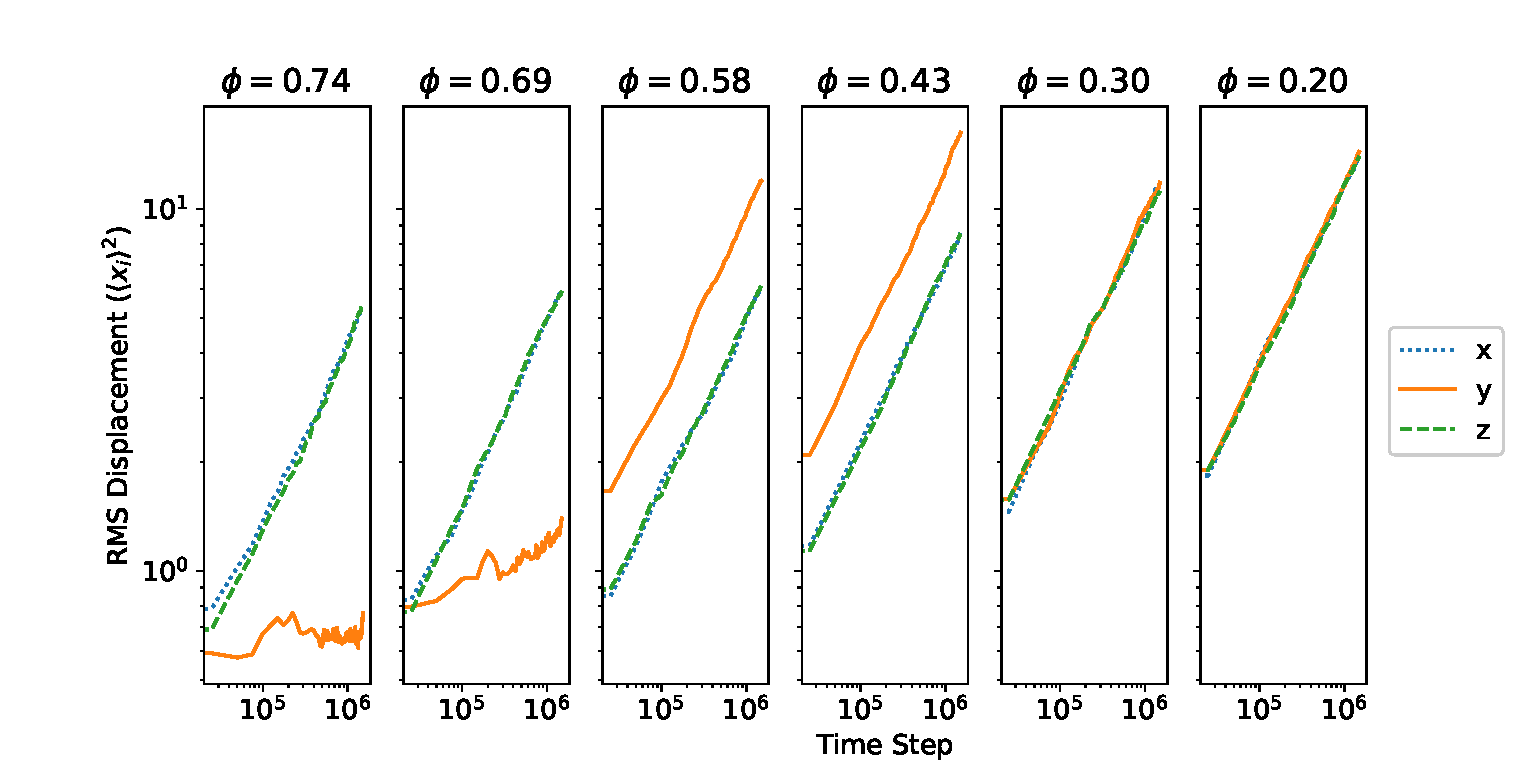
\includegraphics[width=\linewidth]{Figures/nun_diff_rmsplots}
	\caption{Root mean squared (RMS) displacement against time in a system of 1000 rigid rods, for a range of volume fractions $\phi$. The leftmost pair of plots correspond to the smectic phase, with restricted motion between $x-z$ layers along the $y$-axis. The centre pair give the nematic phase, with preferential displacement along the y axis. Finally, the rightmost pair give the isotropic phase, with no preferential direction and isotropic diffusion. Note that there are no significant differences between the $x$ and $z$ directions any phase, as these directions are equivalent in the phase structure.}
	\label{fig:nun_diff_rmsplots}
\end{figure}  %C:\Users\KitG\Documents\LC_Project\Phase_Structure\Nunchucks\Fixed_Angle\Crystalline\Full Transition2

Phase formation may also be observed through deviations in these coordinate-specific diffusion coefficients, measuring the average particle displacement along a given coordinates axes. Here the Cartesian axes may be used, as simulations are configured in a crystalline phase with molecules orientated along the $y$ axis, and smectic layers forming in the $x-z$ plane. Applying this to the nunchucks system, isotropic diffusion is observed at low volume fractions in Figure \ref{fig:nun_diff_Dcoeff}, but the $y$-coordinate diffusion coefficient is severely reduced before this. This strongly indicates the onset of formation of the smectic phase below $\phi = 0.45$, in agreement with the prediction of $ 0.40<\phi^{*}<0.44$ obtained from the smectic order parameter. There is also some indication of the crystalline phase at the highest volume fractions, with diffusion now equally limited in all directions, but this evidence is not conclusive.

\begin{figure} [h!]
	\centering
	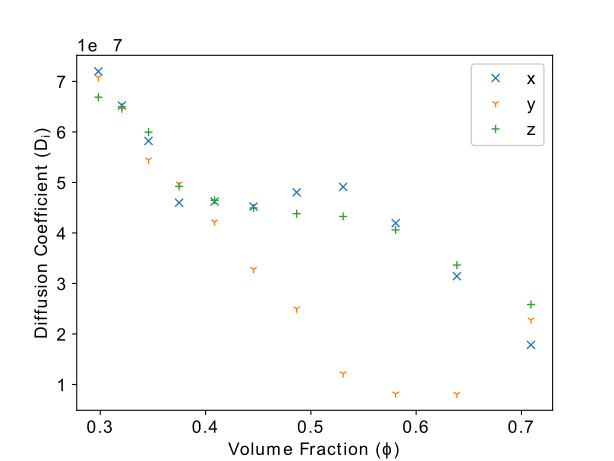
\includegraphics[width=0.7\linewidth]{Figures/nun_diff_Dcoeff}
	\caption{Coordinate diffusion coefficients for the evolution of the microcanonical ensemble under a range of volume fractions $\phi$. The low volume fraction region on the left of the graph corresponds to the isotropic phase, with no variation between coordinate axes. By contrast, the smectic phase in the high volume fraction gives rise to anisotropy in the coordinate diffusion coefficients, with reduced diffusivity perpendicular to the smectic layers in the $y$ axis direction.}
	\label{fig:nun_diff_Dcoeff}
\end{figure}  %C:\Users\KitG\Documents\LC_Project\Phase_Structure\Nunchucks\Fixed_Angle\Crystalline\Full Transition2


%Go on to david's theories for dilute and semi-dilute systems? \textit{also review onsager definitions here?}

\section{Conclusion}
%Summarise key results from above, and emphasise their importance 
%Also give limitations of results obtained, and suggest direction for further work (for each section?)

We considered the phase behaviour of DNA nunchuck molecules, consisting of two sections of ds-DNA connected by a short section of ss-DNA. We introduced a coarse-grained model of DNA nunchuck particles, formed of two rigid rods connected by a (semi-) flexible linker, with soft-core purely repulsive potential interactions. We also introduced a simpler `rigid rod' model, without the flexible linker, to verify the phase identification techniques used here.

Simulations of rigid rods demonstrated the existence of a first-order isotropic\textendash nematic phase transition, and verified Onsager's across a range of aspect ratios. Within this, we confined the critical volume fraction for rods of aspect ratio $D/L = 10$ to the range $0.39<\phi<0.44$, in good agreement with the theoretical value of $\phi = 0.4$. We also considered simulations sampling decreasing volume fractions from an initial crystalline phase, which confirmed the value of this critical volume fraction, verifying the transition occurred at true equilibrium by eliminating the possibility of phase hysteresis here. We also identified the formation of a smectic phase here, however further categorisation of the transitions associated with this phase is left for a separate work.

Application of the same techniques to the nunchucks system gave incontrovertible evidence for the formation of an ordered, quasi-nematic phase in this system, in both the fixed rigidity and fixed angle configurations. The fixed rigidity configuration, a better representation of the true system, demonstrated clear evidence for an entropically-driven phase transition, through the reduction in configurational entropy associated with the formation of a preferred angle. However, further analysis of this system suggested that any periodic order (associated with a novel phase) occurred on a length scale greater than could be simulated here, due to the associated computational costs.

While this is recommended for future work, we instead focus here on the fixed angle configuration, with the aim that restricting the maximum opening angle also reduced the length scale of any periodic order present. We observed the formation of a quasi-nematic phase, and introduced the orientational correlation function in order to identify any periodic order in the `herringbone-like' structure observed. While this confirmed the presence of long-range order, we were unable to observe any periodicity here; we suspect that larger statistics and a longer length scale may be required for this due to the inherent stochastic nature of molecule orientation. \textit{Some final simulations may help suggest the precise future direction of work here}

We also demonstrate that the measurement of dynamic properties provide a little-studied alternative method to identify phase transitions and characteristic symmetries of such systems, in comparison with phases previously identified in both the rigid rods and nunchucks systems previously considered. We consider in particular the formation of anisotropic phases through the variation in coordinate diffusion coefficients, such as in the smectic phase where diffusion between the ordered layers is significantly slower than within them. Further research is necessary to extend this beyond the simple Cartesian approach taken here, to allow the identification of novel phases where the global director or symmetry class is not known.


\section*{Acknowledgements}
I wish to thank my project supervisor (Prof Erika Eiser) and my day-to-day supervisor (Mr Jiaming Yu) for their continual teaching, and Prof Daan Frenkel for the kind insights he offered. Particularly I am grateful for initial code provided by Jiaming to run single-stage, rigid-rod simulations, and the method of calculating the orientational correlation function, detailed in Appendix \ref{sec:PairWise_Theory}, which Daan introduced me to.

%\clearpage
\printbibliography

\begin{appendices}

\section{Onsager Theory} \label{sec:OnsagerAppendix}
A detailed and accessible derivation is provided by Doi and Edwards \cite{Doi1988}, and is not replicated in full here. Briefly summarising their method, the free energy of the system is initially expanded in powers of concentration $\nu$, and higher order terms neglected to give the form:

\begin{equation} \label{eq:OnsagerFreeEnergy}
\mathcal{A}[\Psi(\boldsymbol{u})] = \nu k_{B}T \left[ \ln\nu - 1 + \int d\boldsymbol{u} \Psi(\boldsymbol{u}) \ln \Psi(\boldsymbol{u}) + \frac{1}{2} \int d\boldsymbol{u} \int d\boldsymbol{u^{\prime}} \Psi(\boldsymbol{u}) \Psi(\boldsymbol{u^{\prime}}) \beta(\boldsymbol{u}, \boldsymbol{u^{\prime}})  \right]
\end{equation}

where, for rigid rod-like polymers of diameter $D$ and length $L$, $\beta(\boldsymbol{u}, \boldsymbol{u^{\prime}})$ is given by:

\begin{equation}
\beta(\boldsymbol{u}, \boldsymbol{u^{\prime}}) = 2DL^{2} \left\lvert \boldsymbol{u} \times \boldsymbol{u^{\prime}} \right\rvert
\end{equation} 

This expression may be minimised through the use of a Lagrange multiplier, giving a nonlinear integral equation that cannot be solved linearly. Onsager therefore assumed an equilibrium distribution of the form:

\begin{equation}
\Psi(\boldsymbol{u}) = \frac{\alpha}{4\pi\sinh\alpha} \cosh (\alpha \boldsymbol{u} \cdot \boldsymbol{n})
\end{equation}

for molecule direction $\boldsymbol{u}$, arbitrary unit vector $\boldsymbol{n}$ and order parameter $\alpha$ determined by minimising the free energy. When the concentration exceeds a critical value $\nu^{*}$, a secondary minimum in free energy appears for $\alpha \neq 0$, corresponding to a thermodynamically stable ordered nematic phase. This may not immediately indicate an equilibrium state; indeed Onsager recognised that the free energy may be lowered further by macroscopic phase separation (although we do not expect to observe this in the system sizes considered here). 

Numerical calculation gives $\nu^{*}$, from which the critical volume fraction $\phi^{*}$ may be obtained for rigid rods:

\begin{equation}
\nu^{*} = \frac{16}{\pi D L^{2}}, \qquad \phi^{*} = \nu^{*} \frac{\pi D^{2} L}{4} \simeq 4 \frac{D}{L}
\end{equation}


To derive (\ref{eq:OnsagerFreeEnergy}) that we have assumed it is valid to ignore the third (and higher) Virial coefficients. The reduced third virial coefficient scales as $(D/L)\log(L/D)$, and so is relatively small for the systems considered here. While it should be remembered this may introduce some error in the absolute volume fraction for the phase transition, it does not affect the validity of the phases observed themselves.

Despite its importance in simulation, tt is also acknowledged that this is a typically poor model experimentally; primarily because physical systems either have much lower aspect ratios or are not truly rigid \cite{Odijk1985}. In this case, the long-range Maier\textendash Snape theory \cite{Maier1959} is typically used, with the additional benefit that this also accounts for attractive inter-molecular forces. This produces significantly more accurate estimates of the critical volume fraction and the order parameter at the isotropic\textendash nematic transition \cite{Zannoni1979b}.

\section{Nematic Order Parameter} 
\subsection{Theoretical Outline}\label{sec:OrderParamTheory}
Here I endeavour to outline the motivation for the nematic order parameter used throughout this report, based on the work of Eppenga and Frenkel \cite{Eppenga1984, Frenkel1982}. The nematic phase may be differentiated from the isotropic phase by the formation of cylindrical symmetry, as opposed to the spherical symmetry of the isotropic phase. The deviation from spherical symmetry may be quantified through a set of order parameters \cite{Zannoni1979}. When considering the axially symmetric nematic phase, independent of $\phi$, the distribution function $f(\theta, \phi)$ may be generally expressed in the basis of all even Legendre polynomials $P_{2l}$:

\begin{equation}
f(\theta) = \sum_{l=0}^{\infty} a_{2l} P_{2l}(\cos(\theta))
\end{equation}

where $\theta$ is the angle between the molecular orientation and the axis of symmetry of the system. Note that odd-ordered terms are neglected for nonpolar molecules, as the director may point in either of two antiparallel directions and so all odd Legendre polynomials average to zero \cite{Parsons1979}.

In an isotropic phase, $a_{2l}$ vanishes for all $l>0$, so all angular dependence vanishes. More generally,  quantities $\langle P_{2l}(\cos(\theta)) \rangle$ may be used at the order parameter of the system, with the second order term being referred to as the nematic order parameter. Averaging over a population of $N$ molecules, we can therefore write the nematic order parameter $S_{n}$ as:

\begin{equation}
S_{n} = \frac{1}{N} \left\langle \sum_{i=1}^{N} \left( \frac{3}{2} \cos^{2}(\theta_{i})-\frac{1}{2} \right) \right\rangle
\end{equation}

\subsection{Calculation}\label{sec:OrderParamCalc}
The method given above in Appendix \ref{sec:OrderParamTheory} relies on knowledge of the system-wide nematic director (ie the axis of symmetry of the cylindrical phase), to define $\theta_{i}$. However, this is not always possible in physical systems where such a unique direction is not externally imposed.

Instead, as detailed by Frenkel et al. \cite{Frenkel1985}, we maximise the expression:

\begin{equation} \label{eq:FrenkelNemOrder}
S^{\prime}_{n}(\boldsymbol{\hat{n}^{\prime}}) = \frac{1}{N} \left[ \sum_{i=1}^{N} \left( \frac{3}{2} (\boldsymbol{\hat{n}^{\prime}} \cdot \boldsymbol{\hat{u}_{i}})^{2}-\frac{1}{2} \right) \right]
\end{equation}

where $\hat{u_{i}}$ denotes the orientation of the individual molecular axes in the laboratory frame, and $(\boldsymbol{\hat{n}^{\prime}})$ is the direction of common alignment, known as the director. In the absence of an electric field, the direction of this is arbitrary, and determined in practice by infinitesimal perturbations to the system though spontaneous symmetry breaking \cite{Forster2018}. (\ref{eq:FrenkelNemOrder}) may be further simplified to:

\begin{equation}
S^{\prime}_{n} = \frac{1}{N} \left\langle \boldsymbol{\hat{n}^{\prime}} \cdot \textbf{Q} \cdot \boldsymbol{\hat{n}^{\prime}}  \right\rangle, \qquad where \enspace \textbf{Q}_{i} = \frac{3}{2} \boldsymbol{\hat{u}_{i}}\boldsymbol{\hat{u}_{i}}-\frac{1}{2}\textbf{I}
\end{equation}

The tensor order parameter $\langle \textbf{Q} \rangle$ is a traceless symmetric 2nd-rank tensor, with three eigenvalues $\lambda_{+}, \lambda_{0}, \lambda_{-}$ \cite{Eppenga1984}. We typically take the largest eigenvalue $(\lambda_{+})$ as the nematic order parameter, a good approximation in large N limit.
In practice, we actually calculate the eigenvalues of the related tensor $\textbf{M}$:

\begin{equation}
\textbf{M} =  \frac{1}{N} \sum_{i=1}^{N} \boldsymbol{\hat{u}_{i}}\boldsymbol{\hat{u}_{j}}
\end{equation}

as this shares eigenvectors with $\textbf{Q}$, and has eigenvectors $\mu_{n}$ related to $\lambda_{n}$ by: $\mu_{n} = 2/3 \lambda_{n} + 1/3$.

It is worth noting $\lambda_{+}$ is bound above zero, and so does not reach zero in the isotropic phase as would be expected. It is common to use $S =  -2\lambda_{0}$ when considering such disordered systems, as this fluctuates about an average much closer to zero \cite{Mountain1977}. I have not done so in the results presented here, to give continuity in the order parameter over the transition (wherein lies the focus of this report), however this has meant that the average order parameter in the isotropic phase is slightly above zero.

\subsection{Position Dependant Order Parameter} \label{sec:PairWise_Theory}
The pairwise orientational correlation function, introduced in Section \ref{sec:PairWise_Application} and given in equation (\ref{eq:PairWise_eq}), provides an equivalent to the nematic order parameter that is position dependant. For use in simulation, we rewrite this for $N$ particles in the form:

\begin{equation}
g_{l}(r) = \frac{\sum_{i=1}^{N} \sum_{j \neq i} P_{l}(\boldsymbol{\hat{u}_{i}}\cdot \boldsymbol{\hat{u}_{j}}) \Delta(r_{ij}-r)}{\sum_{i=1}^{N} \sum_{j \neq i} \Delta(r_{ij}-r)}
\end{equation}

where $\Delta(r_{ij}-r) = 1$ if $r_{ij}$ is inside a spherical shell between $r$ and $r+\delta$, and $0$ otherwise. The thickness of $\delta$ is chosen to maximise the resolution of the function, as too large a value will `wash out' important features, while still maintaining a reasonable sample size. This method is very computationally expensive however, as the number of times $P_{L}$ must be calculated scales as $\mathcal{O}(N^{2})$. Furthermore, the storage of all necessary angles is prohibitively expensive (even on modern computers), and limits the resolution possible here \cite{Soper1998}. We may however avoid this problem by expanding the function in terms of spherical harmonics, and sum the contributions for all pairs to a given molecule \cite{Soper1994}. This is most easily done through application of the spherical harmonics addition theorem:

\begin{equation}
P_{l}(\cos \theta_{ij}) = \frac{4\pi}{2l+1} \sum_{m=-l}^{l} \mathcal{Y}_{lm}(\boldsymbol{\hat{u}_{i}}) \mathcal{Y}_{lm}^{*}(\boldsymbol{\hat{u}_{j}})
\end{equation}

Using this, recognising that $\boldsymbol{\hat{u}_{i}}\cdot \boldsymbol{\hat{u}_{j}} = \cos \theta_{ij}$ and writing  $\Delta(r_{ij}-r) = \Delta_{r}$ for simplicity, we may write the contribution from all particles around particle $i$ as:

\begin{equation}
\sum_{i \neq j} P_{l}(\cos \theta_{ij}) \Delta_{r} =  \frac{4\pi}{2l+1} \sum_{j \neq i} \sum_{m=-l}^{l} \mathcal{Y}_{lm}(\boldsymbol{\hat{u}_{i}}) \mathcal{Y}_{lm}^{*}(\boldsymbol{\hat{u}_{j}}) \Delta_{r}
\end{equation}

Exchanging the order of summation, and removing $\mathcal{Y}_{lm}(\boldsymbol{\hat{u}_{i}})$ from the sum over $j$ gives:

\begin{equation}
\sum_{i \neq j} P_{l}(\cos \theta_{ij}) \Delta_{r} =  \frac{4\pi}{2l+1} \sum_{m=-l}^{l} \mathcal{Y}_{lm}(\boldsymbol{\hat{u}_{i}}) \sum_{j \neq i}  \mathcal{Y}_{lm}^{*}(\boldsymbol{\hat{u}_{j}}) \Delta_{r}
\end{equation}

This may be simplified further to:

\begin{equation} \label{eq:pairwise_finalres}
\sum_{i \neq j} P_{l}(\cos \theta_{ij}) \Delta_{r} =  \frac{4\pi}{2l+1} \sum_{m=-l}^{l} \mathcal{Y}_{lm}(\boldsymbol{\hat{u}_{i}}) \times C_{lm}^{*}
\end{equation}

where we have defined

\begin{equation}
 C_{lm}^{*} = \sum_{j \neq i}  \mathcal{Y}_{lm}^{*}(\boldsymbol{\hat{u}_{j}}) \Delta_{r}
\end{equation}

This removes the requirement to calculate $P_{l}$ for every pair of molecules, in favour of simply summing the spherical harmonics terms corresponding to a given shell around $i$, then multiply spherical harmonics components. It should also be noted that (\ref{eq:pairwise_finalres}) is invariant under changes in the coordinate frame; in our computations all orientations were expressed in the lab frame for each (rather than aligning the coordinate frame with the global director).

\section{Mean Squared Displacement} \label{sec:Diffusion_Theory}
Here, we provide a derivation of the diffusion relation (\ref{eq:msd_eq}), taking a popular approach through the derivation of the moment generating function \cite{Mazo2008, Gardiner2009}. The diffusive motion of a particle is a stochastic process, which may be described by a probability density function (PDF) that satisfies the diffusion equation:

\begin{equation} \label{eq:diff_eq}
\frac{\partial p(x,t \mid x_{0})}{\partial t} = D\frac{\partial^{2} p(x,t \mid x_{0})}{\partial x^{2}}
\end{equation}

where $x(t)$ is the position of the particle at some time $t$, and $x_{0}$ is the initial position of the particle. For simplicity we will use a one dimensional space here, but the argument is easily extended to higher dimensions. 

This is trivially obeyed by the Green's function $G(x,t)$, where this is defined to be the time evolution of density $G(x,0)=\delta(x)$ (taking $x_{0} = 0$ for simplicity). We must therefore first obtain $G(x,t)$ for which we will use Fourier transform methods based on the approach by Sethna \cite{Sethna2006}. In general, we may decompose our solution into a family of plane wave solutions of the form $\tilde{p}_{k}(t)e^{ikx}$. Substituting this into (\ref{eq:diff_eq}), we obtain

\begin{equation}
\frac{\partial p}{\partial t} = \frac{d\tilde{p}_{k}}{dt}e^{ikx} =  D\frac{\partial^{2}p}{\partial x^{2}} = -Dk^{2}\tilde{p}_{k}(t)e^{ikx}
\end{equation}

from which we may extract a differential equation in $\tilde{p}_{k}(t)$, with the simple solution:

\begin{equation} \label{eq:Fourier_wave}
\tilde{p}_{k}(t) = \tilde{p}_{k}(0)e^{-Dk^{2}t}
\end{equation}

The Fourier transform of $G(x,t)$ at $t=0$ is given by:

\begin{equation}
\tilde{G}_{k}(0) = \int G(x,0)e^{-ikx}dx = \int \delta(x)e^{-ikx}dx = 1
\end{equation}

and so the time dependant Fourier transform is given by $\tilde{G}_{k}(t) = e^{-Dk^{2}t}$ according to (\ref{eq:Fourier_wave}). This gives a the real-space $G(x,t)$ as:

\begin{equation}
G(x,t) = \frac{1}{2\pi} \int e^{ikx} \tilde{G}_{k}(0)e^{-Dk^{2}t}dk = \frac{1}{2\pi} \int e^{ikx} e^{-Dt^{k}t}dk
\end{equation}

This is simply the inverse Fourier transform of a Gaussian, and so evaluates to:

\begin{equation}
G(x,t) = \frac{1}{\sqrt{4\pi Dt}}e^{-x^{2}/4Dt}
\end{equation}

Redefining the spatial coordinate to account for the initial conditions, the probablility density function is given by:

\begin{equation}
P(x,t) = \frac{1}{\sqrt{4\pi Dt}}e^{-(x-x_{0})^{2}/4Dt}
\end{equation}

Using this function, the average of an arbitrary function $A$ at time $t$ is given by:

\begin{equation}
\langle A(t) \rangle = \int_{-\infty}^{\infty} A(x,t)P(x,t) dx
\end{equation}

This must be evaluated for the mean squared displacement (MSD):

\begin{equation} \label{eq:MSD_theory} 
\langle (x(t) - x_{0})^{2} \rangle = \langle x^2 \rangle + x_{0}^{2} -2x_{0}\langle x \rangle 
\end{equation}

 
While it is possible to evaluate $\langle x \rangle$ and $\langle x^2 \rangle$ explicitly, it is perhaps more elegant to find the moment generating function, which describes the $k$-th moment of the PDF. We first introduce the characteristic function:

\begin{equation} \label{eq:characteristic_func}
\phi_{x}(k) = \langle e^{ikx} \rangle = \int e^{ikx} P(x,t \mid x_{0}) dx = \sum_{n=0}^{\infty} \frac{(ik)^{n}}{n!}\langle x^{n} \rangle
\end{equation}

where $\langle x^{n} \rangle$ are the moments of $P(x)$. We may separately define the cumulants $C_{n}$ by writing $\phi_{x}(k)$ in the form (the motivation for which will shortly be apparent):

\begin{equation}
\phi_{x}(k) =  \exp \left[\sum_{n=0}^{\infty} \frac{(ik)^{n}}{n!} C_{n}  \right]
\end{equation}

Comparing coefficients with (\ref{eq:characteristic_func}), we may identify the cumulants explicitly as:

\begin{equation}
C_{n} = \frac{d^{n}}{d(ik)^{n}} \ln \left(\phi_{x}(k) \right) \biggr|_{k=0} 
\end{equation}

As (\ref{eq:characteristic_func}) may be evaluated by completing the square to give the form:

\begin{equation}
\phi_{x}(k) = e^{ikx_{0} - k^{2}Dt}
\end{equation}

we find by simple substitution that the first two cumulants are given by:

\begin{equation}
C_{1} = x_{0}, \qquad C_{2} = 2Dt
\end{equation}

Note that this value for $C_{1}$ is expected, as it corresponds to the mean of the Gaussian distribution. Substitution of these values into (\ref{eq:MSD_theory}) renders the desired result:

\begin{equation}
\langle (x(t) - x_{0})^{2} \rangle = 2Dt
\end{equation}








\section{Code?}

\end{appendices}

\end{document}


%%%%%%%%%%%%%%%%%%%%%%%%%%%%%%%%%%%%%%%%%
% Wenneker Article
% LaTeX Template
% Version 2.0 (28/2/17)
%
% This template was downloaded from:
% http://www.LaTeXTemplates.com
%
% Authors:
% Vel (vel@LaTeXTemplates.com)
% Frits Wenneker
%
% License:
% CC BY-NC-SA 3.0 (http://creativecommons.org/licenses/by-nc-sa/3.0/)
%
%%%%%%%%%%%%%%%%%%%%%%%%%%%%%%%%%%%%%%%%%
